% =====================================================================
% ROZDZIAŁ 4 — Lateral phishing jako naruszenie grafu komunikacji
% (na bazie artykułu A, JNCA; liczby wprost z code/results/*.csv)
% =====================================================================
\chapter{Lateral phishing jako naruszenie grafu komunikacji organizacji}
\label{rozd:kaskada}

\section{Teza cząstkowa i plan rozdziału}
\label{sec:k-teza}

Ten rozdział rozwija i sprawdza pierwszą połowę tezy T1: lateral
phishing --- kampania wysłana z przejętego konta wewnętrznego --- jest
naruszeniem \emph{grafu komunikacji organizacji w czasie}. Przejęte
konto przechodzi każdą kontrolę statyczną (tożsamość, reputacja,
relacja), bo wszystkie one są prawdziwe; naruszenie leży w dwóch
miejscach, których żaden filtr treści nie widzi. Po pierwsze, konto
pisze poza własnym rytmem. Po drugie --- i to jest decydujące ---
atak \emph{propaguje}: kaskada zostawia po stronie odbiorców falę ---
w krótkim oknie wiele kont w jednym otoczeniu jest trafionych, każde
przez nadawcę trafionego chwilę wcześniej --- której żadna pojedyncza
wiadomość nie zdradza. Teza jest testowalna przez RQ1 (sygnał) i RQ2
(granice) z rozdziału~\ref{rozd:wstep}.

Plan: sekcja~\ref{sec:k-model} formalizuje graf komunikacji i model
zagrożeń kaskady; sekcja~\ref{sec:k-detektory} buduje hierarchię
detektorów rosnącej świadomości temporalnej; sekcja~\ref{sec:k-protokol}
wiąże protokół ewaluacji z warunkami rozdziału formalnego;
sekcja~\ref{sec:k-studium} stanowi studium przypadku; wyniki --- od
hierarchii detektorów, przez atakującego skrytego, granice modelu
zagrożeń, stabilność, walidację na realnych grafach po rygor
ewaluacji --- zajmują sekcje~\ref{sec:k-hierarchia}--\ref{sec:k-rygor};
sekcja~\ref{sec:k-podsumowanie} podsumowuje odpowiedzi na RQ1--RQ2.
Granica modelu zagrożeń jest ustalona jawnie: pojedyncza, chirurgiczna
wiadomość od przejętego konta do jednego odbiorcy --- klasyczna prośba
„CEO do CFO" o przelew --- nie propaguje i nie zostawia fali; jest to
punkt ślepy \emph{wszystkich} badanych detektorów (sekcja
\ref{sec:k-granice}) i pozostaje domeną kontroli procesowych poza
pasmem kanału komunikacji.

\section{Model: graf komunikacji i kaskada}
\label{sec:k-model}

Obiektem monitoringu jest \emph{graf komunikacji} organizacji:
$G=(V,E)$, gdzie $V$ to konta, a $E$ to kontakty (kto z kim
koresponduje), wzbogacony o \emph{rytm} $\tau\colon V\to\mathcal{T}$
przypisujący każdemu kontu zbiór aktywnych okien czasowych. Czas jest
dyskretyzowany na kubełki (sekcja~\ref{sec:k-studium}); zdarzenia
$(s,v,b)$ --- nadawca, odbiorca, kubełek --- są instancją strumienia
z definicji~\ref{def:stream}, a porządek totalny $t(\event)=(b,\rho)$
i historia własna $H_{\strict\event}$ --- z rozdziału
formalnego. Detektory są budowane wyłącznie z cech
zdarzeniowo-przyczynowych w sensie definicji~\ref{def:causal-feature}:
liczniki wolumetryczne i pamięć modelu temporalnego widzą wyłącznie
zdarzenia o \emph{ściśle wcześniejszym} znaczniku czasu; jest to
konsekwencja napraw wycieków opisanych w rozdziale~\ref{rozd:wstep}
(każda cecha strumieniowa liczona wyłącznie z przeszłości, zgodnie
z pamięcią modelu temporalnego).

\paragraph{Model zagrożeń.} Atak to kaskada: przejęte konto
$s_0$ (patient zero) wysyła złośliwą pocztę do swoich kontaktów;
każdy odbiorca staje się nosicielem z prawdopodobieństwem
$p_{\mathrm{inf}}$ i propaguje dalej do głębokości $H$. Pojedyncze
zdarzenie $u\!\to\!v$ jest \emph{lokalnie} nieodróżnialne od legalnej
poczty od znanego kontaktu; sygnałem jest kontekst kaskadowy: w oknie
fali wielu sąsiadów $v$ otrzymuje pocztę, a $u$ było trafione
właśnie przedtem. Rozważamy trzy reżimy ataku, każdy dobrany tak, by
przeciążyć konkretne twierdzenie, a nie by reprezentować typowy
ruch:
\begin{enumerate}
\item \emph{kaskada domyślna} ($p_{\mathrm{inf}}=0{,}6$, $H=4$):
reżim bazowy hierarchii detektorów;
\item \emph{atak skryty} ($K$ nosicieli, jedna wysyłka na kubełek,
aż do $K{=}1$): burst nadawczy jest rozsmarowany w czasie --- reżim,
który \emph{łamie} detekcję wolumetryczną i izoluje sygnał
odbiorczy; zgodnie ze stwierdzeniem~\ref{prop:withinbucket} liczniki
wolumetryczne --- przyczynowe zdarzeniowo --- widzą rozwijający się
burst dopóki jego zdarzenia mieszczą się w kolejnych kubełkach;
\item \emph{atak chirurgiczny} ($p_{\mathrm{inf}}=0$, fan-out 1):
brak jakiejkolwiek propagacji --- mierzony punkt ślepy (RQ2).
\end{enumerate}
Ruch legalny to poczta między znanymi kontaktami w rytmie, z frakcją
przychodzącą poza rytm (nieodwracalne źródło fałszywych alarmów)
oraz frakcją ataków mimikujących rytm --- dwustronny szum, by klasy
nie były idealnie rozdzielne.

\section{Detektory: hierarchia świadomości temporalnej}
\label{sec:k-detektory}

Zasada projektowa jest jednolita: cechy kodują pozycję w grafie
i czas, \emph{nigdy tożsamość} --- dzięki temu każdy detektor jest
indykcyjny (zastosowalny do kont niewidzianych w treningu). Porównujemy
detektory o rosnącej świadomości temporalnej:

\begin{itemize}
\item \textbf{1-hop (tabular)}: lokalne cechy pojedynczego zdarzenia ---
dolne ograniczenie;
\item \textbf{ręczny kontekst kaskadowy}: cechy ręczne 1-hop plus
gęstość fali (liczba kontaktów ofiary trafionych w oknie),
świeżość nadawcy (freshness) i burst;
\item \textbf{GNN statyczny}: topologia zagregowanego grafu, bez czasu;
\item \textbf{GNN temporalny z pamięcią węzłów}: pamięć aktualizowana
kubełek po kubełku, czytana kubełek \emph{przed} zdarzeniem, które
ocenia --- zachowuje przyczynowość (def.~\ref{def:causal-detector});
\item \textbf{COMPA (wolumetryczny)}: odchyłka nadawcy od własnego
profilu wolumetrycznego --- nowość odbiorcy, nowość kubełka,
aktywność nadawcy;
\item \textbf{hopper (path-based)}: transfer idei ścieżki przyczynowej
Hoppera \citep{ho2021hopper} na graf poczty: prekursor, momentum,
rzadki cel.
\end{itemize}

Dwa równania pokazują, gdzie mieszka różnica. Statyczny detektor
buduje osadzenia z zagregowanego grafu ze znormalizowaną
incydencją $\hat A$ i cechami $X$,
\begin{equation}
Z = \hat{A}\,\sigma\!\big(\hat{A}\,X\,W_1\big)\,W_2,
\qquad
\mathrm{score}_{\mathrm{stat}}(s,v) =
g\!\big([\,Z_s,\,Z_v,\,Z_s\!\odot\!Z_v,\,x_{sv}\,]\big),
\label{eq:k-static}
\end{equation}
widząc, kto z kim jest połączony, ale nie w jakiej kolejności.
Temporalny utrzymuje pamięć $m_v^{(b)}$ i ocenia zdarzenie kubełka
$b$ stanem \emph{sprzed} jego aktualizacji:
\begin{align}
\mathrm{score}_{\mathrm{temp}}(s,v,b) &=
g\!\big([\,m_s^{(b-1)},\,m_v^{(b-1)},\,
m_s^{(b-1)}\!\odot\!m_v^{(b-1)},\,x_{sv}\,]\big),
\label{eq:k-tempscore}\\
m_v^{(b)} &= \mathrm{GRU}\!\Big(\tfrac{1}{d_v^{(b)}}
\!\!\sum_{u:\,(u\to v)\in b}\!\!
\sigma\!\big(W_m\,m_u^{(b-1)}\big),\; m_v^{(b-1)}\Big),
\label{eq:k-tempmem}
\end{align}
gdzie $d_v^{(b)}$ to in-stopień $v$ w kubełku $b$. To właśnie
odczytywanie pamięci sprzed aktualizacji pozwala fali odbiorczej
stać się sygnałem --- i to właśnie tasowanie czasu niszczy
(stw.~\ref{prop:shuffle}). Jako sanity-check architektury porównujemy
też biblioteczną implementację TGN \citep{rossi2020temporal}
(wartości w sekcji~\ref{sec:k-hierarchia}); modele trenujemy
z ustalonymi jednolicie hiperparametrami, bez intensywnego
strojenia, tak by żaden detektor nie miał przewagi strojenia.

\section{Protokół ewaluacji: cztery zabezpieczenia}
\label{sec:k-protokol}

Grafowe detektory łatwo zawyżyć, dlatego protokół stosuje cztery
zabezpieczenia, z których każde jest instancją warunku z rozdziału
formalnego:
\begin{enumerate}
\item \emph{projekt dopasowany} (matched design): legalne i atakowe
krawędzie mają ten sam rozkład końców i stopni --- różnią się wyłącznie
wzorcem czasowym; usuwa to konfounder stopnia/tożsamości
\citep{arp2022dos};
\item \emph{kontrola tasowania czasu}: permutacja porządku zdarzeń
niszczy przewagę, jeśli pochodzi ona z dynamiki, a zostawia ją, jeśli
jest artefaktem topologii lub tożsamości \citep{pendlebury2019tesseract};
abelacja jest selektywna tylko w ograniczeniu --- tasowanie psuje też
ko-występowanie wewnątrz kubełka, więc $\Delta_{\mathrm{porz}}$ jest
ograniczeniem \emph{z góry} wkładu samego porządku
(stw.~\ref{prop:shuffle});
\item \emph{podziały}: po ofiarach (rozłączne zbiory ofiar;
stw.~\ref{prop:split}) w badaniach głównych oraz po organizacjach
(walidacja indukcyjna);
\item \emph{metryki operacyjne}: czułość przy niskim FPR
($\alpha=1\%$), z jawną arytmetyką bazy (stw. o~arytmetyce bazy,
rozdz.~\ref{rozd:formalny}), zamiast samego nagłówkowego AUC;
\item \emph{sonda predyktywności}: hierarchia jakościowa detektorów
i kierunek kontrastu głównego (sygnał odbiorczy vs wolumetryczny)
muszą przenieść się na realne topologie; przy kilku ziarnach na graf
to kontrola kierunkowa, nie test istotności.
\end{enumerate}
Liczba ziaren jest podana przy każdej tabeli; wartości per-seed
każdej tabeli są dostępne w paczce reprodukcyjnej.

\section{Studium przypadku: organizacja}
\label{sec:k-studium}

Studium przypadku to w pełni określony ekosystem organizacyjny
(rysunek~\ref{fig:k-casestudy}): $19$ firm z różnych sektorów (bank,
grupa szpitalna, software house, kancelaria, logistyka, ubezpieczyciel,
urząd, \dots), każda małym biurem $\sim\!8$ kont: dyrektor zarządzający,
senior manager i pięciu--sześciu specjalistów i analityków
($19/19/57/55$ kont na czterech poziomach starszeństwa). Każdy
koresponduje z każdym w swojej firmie, a firmy są spięte w pierścień
partnerstw biznesowych (dyrektor z dyrektorem plus po jednym
kontrahencie specjalistycznym), co daje $N{=}150$ kont i $556$
krawędzi kontaktów ($518$ wewnątrz firm, $38$ między partnerami).
Populacja jest syntetyczna, ale wygenerowana \emph{graph-first}:
schemat organizacji ustalony deterministycznie, każda persona wpisana
w swój węzeł, tak że przełożony, współpracownicy i kontakty zewnętrzne
persony to \emph{realne inne persony}, a graf domyka się wewnętrznie.
Skala $N{=}150$ jest rzędu rdzenia użytkowników korpusu Enron
\citep{klimt2004enron}; graf kontaktów Enron użyty do walidacji jest
większy ($\sim\!1970$ kont), więc replikacja realna testuje też
mechanizm w większej skali.

Tydzień dzielimy na $T{=}28$ kubełków (7 dni $\times$ 4 bloki
sześciogodzinne); rytm konta to zbiór jego aktywnych kubełków
(syntetycznie 6 na personę; na Enronie wyprowadzony z nagłówków
\texttt{Date}). Realistyczny szum: $15\%$ legalnej poczty przychodzi
poza rytmem, $25\%$ ataków mimikuje rytm. Kaskada domyślna:
$p_{\mathrm{inf}}{=}0{,}6$, głębokość $H{=}4$.

\begin{figure}[htbp]\centering
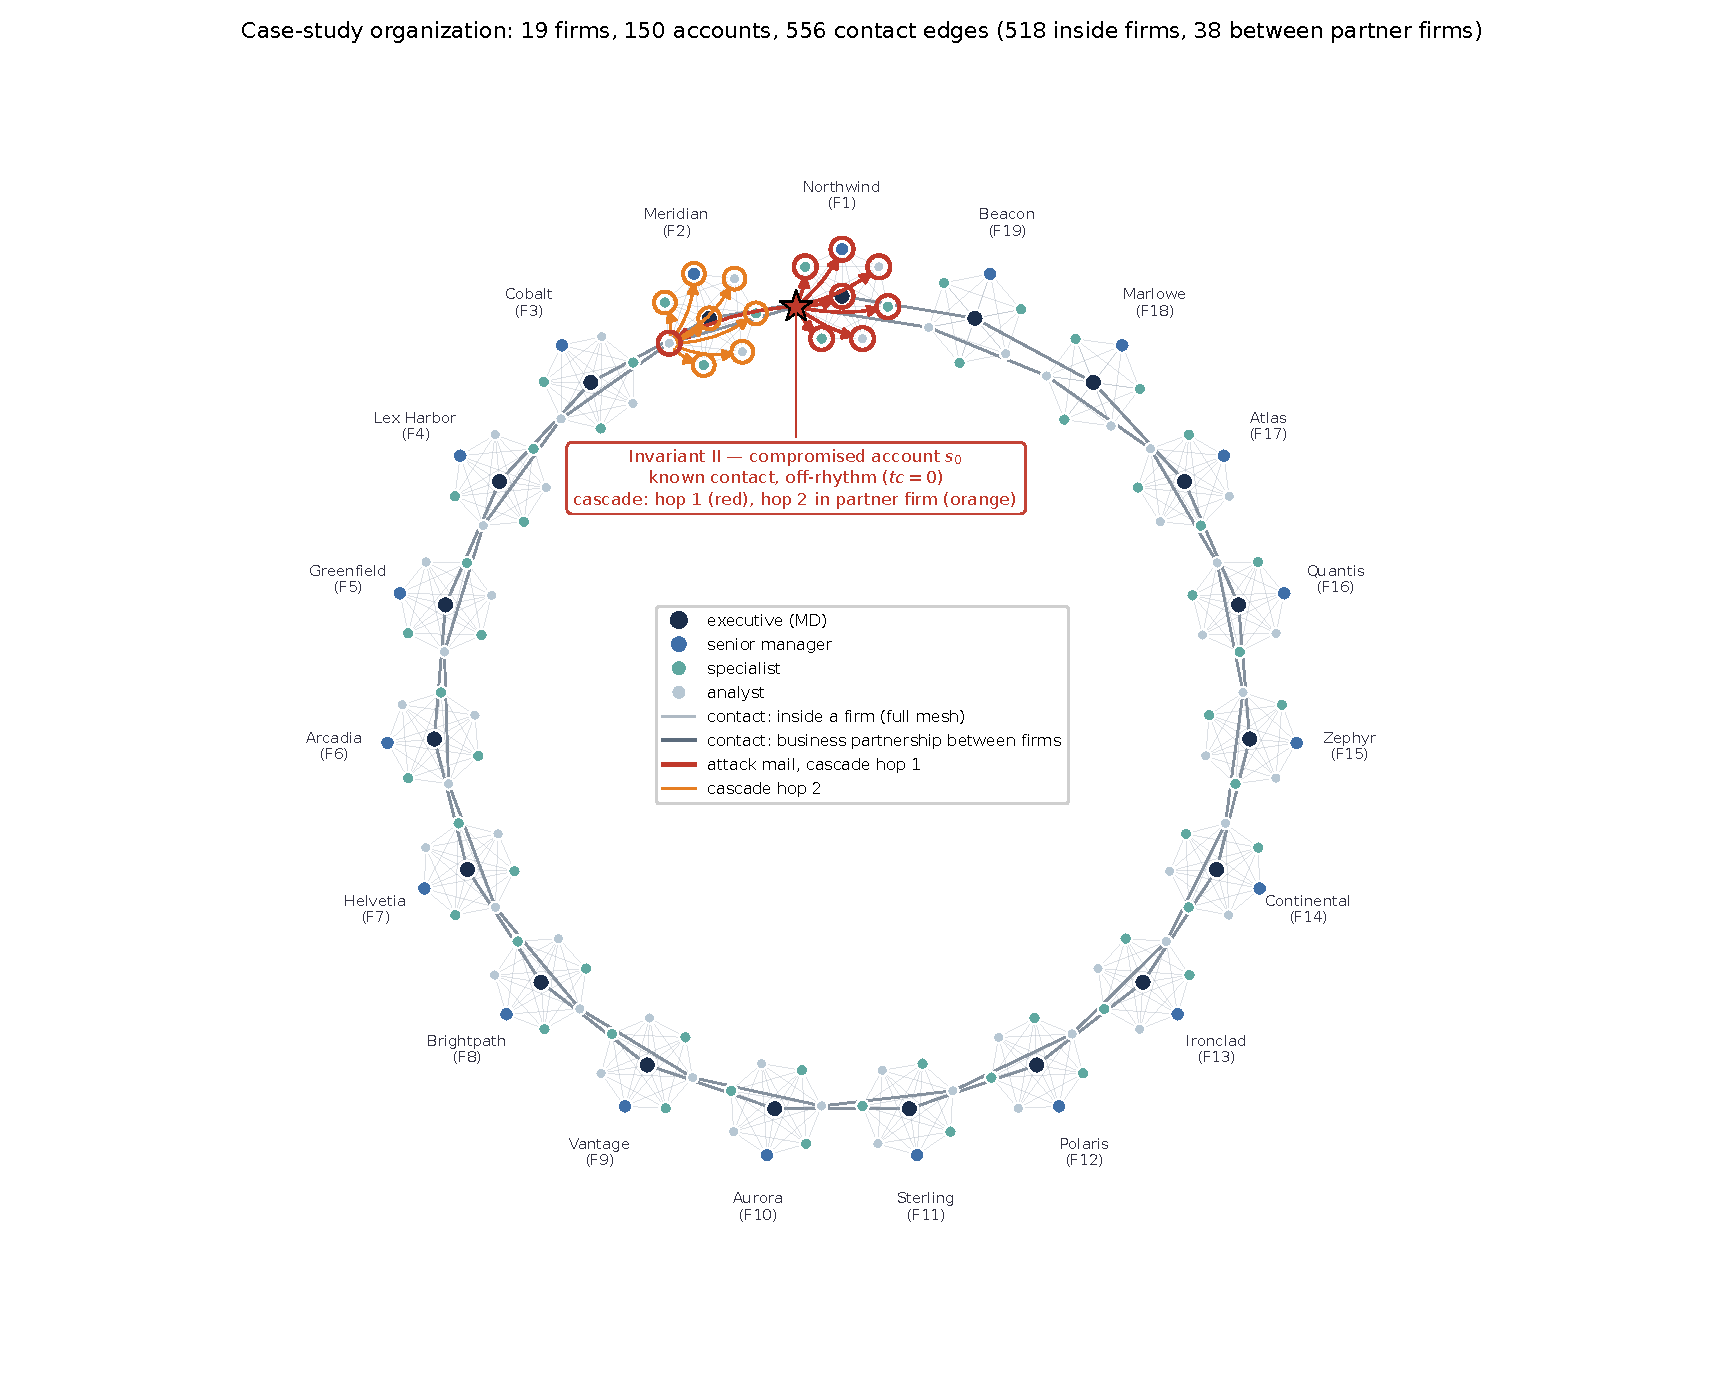
\includegraphics[width=0.95\textwidth]{fig_org_case_study_cascade.pdf}
\caption{Organizacja studyjna z danych populacji paczki
reprodukcyjnej: $19$ firm na pierścieniu partnerstw, $150$ kont
kolorowanych po starszeństwie, warstwa kontaktów ($556$ krawędzi).
Nałożony atak, który detektory muszą wykryć: przejęte konto $s_0$
(gwiazdka), którego poczta poza rytmem kaskadowa się przez własną
firmę (hop~1, czerwony) i przez krawędź partnerską do firmy sąsiedniej
(hop~2, pomarańczowy). Każda wiadomość kaskady pochodzi od realnego
kontaktu; zdradzają ją wyłącznie czas i fala po stronie odbiorców.}
\label{fig:k-casestudy}
\end{figure}

\section{Wyniki: hierarchia detektorów}
\label{sec:k-hierarchia}

Przejęte konto przechodzi każdą relację statyczną, więc sama pozycja
w grafie niesie mało sygnału operacyjnego: GNN statyczny osiąga AUC
$0{,}76$, ale czułość@FPR$1\%$ tylko $0{,}039$
(tab.~\ref{tab:k-detektory}). Sygnał musi więc mieszkać w dynamice.
Tabela~\ref{tab:k-detektory} testuje T1 na kaskadzie domyślnej
i pokazuje wyraźną hierarchię: lokalne cechy 1-hop są bezużyteczne
(AUC $0{,}70$, czułość $\approx 0$), ręczny kontekst kaskadowy
i detektor wolumetryczny COMPA czytają sygnał burstu ($0{,}81$,
odpowiednio $0{,}83$), a temporalny GNN z pamięcią węzłów prowadzi
(AUC $0{,}87$, czułość@FPR$1\%$ $0{,}099$). Przewaga jest temporalna
w sensie ablacyjnym: proste tasowanie porządku czasu cofa model
temporalny do poziomu statycznego ($0{,}87\to0{,}73$; czułość
$0{,}099\to0{,}022$), zgodnie ze stwierdzeniem~\ref{prop:shuffle}.
Wybór architektury znaczy mniej niż paradygmat: TGN-lite wyprzedza
ręczny kontekst we wszystkich ziarnach, a biblioteczny TGN
\citep{rossi2020temporal} dorównuje mu na metryce operacyjnej
(czułość@1\% $0{,}112$ wobec $0{,}078$ TGN-lite przy AUC $0{,}79$
wobec $0{,}85$; 3 ziarna).

\begin{table}[htbp]\centering
\begin{tabular}{lcc}
\toprule
Detektor & AUC & czułość@FPR$1\%$ \\
\midrule
1-hop (tabular)            & $0{,}70$ & $0{,}006$ \\
GNN statyczny              & $0{,}76$ & $0{,}039$ \\
Ręczny kontekst (tab.)     & $0{,}81$ & $0{,}023$ \\
COMPA (wolumetryczny)      & $0{,}83$ & $\mathbf{0{,}232}$ \\
\textbf{GNN temporalny}    & $\mathbf{0{,}87}$ & $0{,}099$ \\
GNN temporalny (tasowany)   & $0{,}73$ & $0{,}022$ \\
\bottomrule
\end{tabular}
\caption{Hierarchia detektorów kaskady na grafie studyjnym (podział
po ofiarach, 5 ziaren; \texttt{exp\_cascade.csv}). Tylko model
temporalny z pamięcią węzłów łączy wysoki AUC z miarą czułości
operacyjnej; COMPA ma wysoką czułość na tym reżimie, bo jej
przyczynowo-zdarzeniowe liczniki widzą rozwijający się burst
(wtw.~\ref{prop:withinbucket}), ale załamuje się w reżimie skrytym
(tab.~\ref{tab:k-stealth}). Tasowanie czasu usuwa przewagę
temporalnego.}
\label{tab:k-detektory}
\end{table}

\section{Wyniki: atakujący skryty}
\label{sec:k-stealth}

Tabela~\ref{tab:k-stealth} jest testem głównym T1: atakujący skryty
łamie detekcję wolumetryczną, ale nie dynamikę. Przy atakującym,
który rozkłada wysyłki w czasie ($K$ nosicieli, jedna wysyłka na
kubełek), detektor wolumetryczny traci sygnał: przy $K{=}1$ jego AUC
spada do $0{,}52$ z czułością $0{,}000$ --- burst nadawczy znika,
więc nie ma żadnego wzrostu per-kubełek, który byle jaka statystyka
wolumetryczna mogłaby zobaczyć --- podczas gdy model temporalny
degraduje łagodniej i trzyma się powyżej losowego (AUC $0{,}59$,
czułość $0{,}049$), czytając falę po stronie odbiorców. Przy
$K\to$blast przewaga wolumetryczna wraca ($0{,}63\to0{,}85$
temporalnego). Wartości na tym wykresie (rysunek~\ref{fig:k-stealth})
czytają się jako krzywa: im skrytszy atak, tym mocniej wolumetryczny
się załamuje.

Sam \emph{bit rytmu} nie wnosi nic w tym harnessie: detektor
rhythm-only trzyma AUC $0{,}50$ na każdym poziomie $K$
(tab.~\ref{tab:k-stealth}), bo --- zgodnie z audytem rytmu
(\texttt{exp\_cascade\_stealth\_tc.csv}) --- poczta poza rytmem
to $75$--$79\%$ zdarzeń ataku \emph{i} $78$--$79\%$ ruchu legalnego:
klasy są po rytmie wymienne. Sygnałem jest fala po stronie
\emph{odbiorców}, nie rytm nadawcy --- co jest empiryczną
koniugacją lematu~\ref{lem:probe}: skoro brzeg czasowy nie
rozdziela klas, marża musi pochodzić ze sprzężenia czasu ze
strukturą grafu.

\begin{table}[htbp]\centering
\begin{tabular}{lcccccc}
\toprule
& \multicolumn{2}{c}{COMPA} & \multicolumn{2}{c}{GNN temporalny} & rhythm-only \\
\cmidrule(lr){2-3}\cmidrule(lr){4-5}\cmidrule(lr){6-6}
Poziom & AUC & cz.@1\% & AUC & cz.@1\% & AUC \\
\midrule
$K{=}1$ (ekstremalnie skryty) & $0{,}52$ & $0{,}000$ & $\mathbf{0{,}59}$ & $\mathbf{0{,}049}$ & $0{,}50$ \\
$K{=}2$ & $0{,}58$ & $0{,}011$ & $\mathbf{0{,}72}$ & $\mathbf{0{,}037}$ & $0{,}51$ \\
$K{=}3$ & $0{,}57$ & $0{,}011$ & $\mathbf{0{,}74}$ & $\mathbf{0{,}049}$ & $0{,}50$ \\
$K{=}5$ & $0{,}61$ & $0{,}031$ & $\mathbf{0{,}76}$ & $\mathbf{0{,}044}$ & $0{,}50$ \\
blast & $0{,}63$ & $0{,}030$ & $\mathbf{0{,}85}$ & $\mathbf{0{,}071}$ & $0{,}54$ \\
\bottomrule
\end{tabular}
\caption{Atakujący skryty na grafie studyjnym ($K$ nosicieli
rozłożonych w czasie; 20 ziaren; \texttt{exp\_cascade\_stealth.csv},
timing deterministyczny). W miarę $K\to1$ detektor wolumetryczny
traci cały sygnał (czułość $0{,}000$), podczas gdy sygnał odbiorczy
modelu temporalnego degraduje łagodniej i trzyma się powyżej
losowego --- główny wynik operacyjny za T1. Sam rytm nadawcy
(rhythm-only) jest bezużyteczny na każdym poziomie.}
\label{tab:k-stealth}
\end{table}

\begin{figure}[htbp]\centering
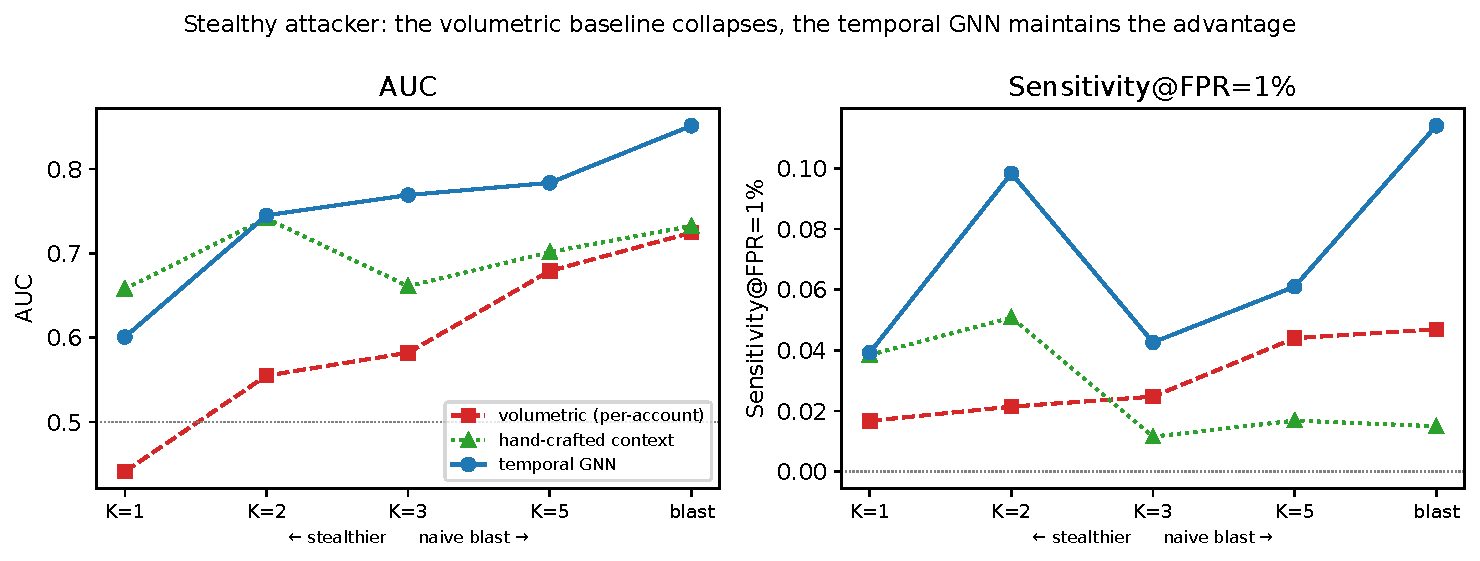
\includegraphics[width=0.9\textwidth]{fig_cascade_stealth.pdf}
\caption{Skrytość a załamanie wolumetryczne: im skrytszy atak
(mniejsze $K$), tym mocniej detektor wolumetryczny się załamuje;
model temporalny degraduje łagodniej dzięki fali po stronie
odbiorców (dane \texttt{exp\_cascade\_stealth.csv}).}
\label{fig:k-stealth}
\end{figure}

\paragraph{Panel baseline'ów.} Tabela~\ref{tab:k-baselines}
stawia ten wynik przeciw dwóm mocnym metodom praktycznym
(harness \texttt{cb}, timing deterministyczny, 20 ziaren). W reżimie
skrytym ręczny kontekst prowadzi przy ekstremalnej skrytości
($K{=}1$: $0{,}77$, przed path-based $0{,}74$ i temporalnym
$0{,}61$), ale traci prowadzenie, gdy tylko kaskada sięga dalej;
path-based degraduje z zasięgiem ($0{,}74\to0{,}65$); a temporalny
GNN jest jedynym detektorem bez reżimu załamania --- w wąskim przedziale
$0{,}61$--$0{,}85$ przez wszystkie poziomy, na prowadzeniu od
$K{=}3$. Ablacja hoppera bez cechy \emph{precursor} pokazuje, że
to właśnie prekursor (odpowiednik świeżości kontekstu ręcznego) niesie
jego sygnał stealth: $0{,}74\to0{,}63$ przy $K{=}1$.

\begin{table}[htbp]\centering\small
\begin{tabular}{lcccccc}
\toprule
Poziom (zasięg) & COMPA & hopper & hopper$\emptyset$prek. & ręczny & temporalny \\
\midrule
$K{=}1$ (11\%) & $0{,}51$ & $0{,}74$ & $0{,}63$ & $\mathbf{0{,}77}$ & $0{,}61$ \\
$K{=}2$ (28\%) & $0{,}58$ & $0{,}70$ & $0{,}63$ & $0{,}69$ & $0{,}68$ \\
$K{=}3$ (46\%) & $0{,}60$ & $0{,}66$ & $0{,}63$ & $0{,}66$ & $\mathbf{0{,}72}$ \\
$K{=}5$ (63\%) & $0{,}64$ & $0{,}65$ & $0{,}64$ & $0{,}68$ & $\mathbf{0{,}77}$ \\
blast (75\%)   & $0{,}70$ & $0{,}82$ & $0{,}79$ & $0{,}75$ & $\mathbf{0{,}85}$ \\
\bottomrule
\end{tabular}
\caption{Panel baseline'ów w reżimie skrytym (AUC, 20 ziaren,
timing deterministyczny; \texttt{cb\_hopper\_stealth.csv}). Ręczny
kontekst prowadzi tylko przy $K{=}1$; hopper degraduje z zasięgiem
(prekursor niesie jego sygnał: $0{,}74\to0{,}63$ po ablacji);
temporalny GNN jest jedynym detektorem bez reżimu załamania.}
\label{tab:k-baselines}
\end{table}

\paragraph{Kontrasty statystyczne.} Wzmocnienie głównego kontrastu
na 20 ziarnach testem Wilcoxona i Cliffa $\delta$
(\texttt{cb\_headline\_contrasts.csv}): sygnał odbiorczy bije detekcję
wolumetryczną istotnie i z dużym efektem (temporalny GNN
$+0{,}115$ AUC, $p<0{,}001$, $\delta=0{,}98$; w protokole benign
empirycznym $+0{,}113$, $\delta=0{,}99$), podczas gdy temporalny
GNN \emph{nie} bije istotnie kontekstu ręcznego ($+0{,}021$,
$p=0{,}19$; w protokole empirycznym $+0{,}002$, $p=0{,}93$):
sygnał odbiorczy czytają równie dobrze model nauczony i cechy
ręczne. Załamanie wolumetryczne nie jest artefaktem strojenia:
COMPA nie ma okna ani progu do strojenia --- jej trzy cechy to
liczniki na obserwowanym strumieniu karmione tym samym learnerem
co każda inna metoda tabularna --- więc załamanie jest własnością
modelu ataku: jedna wysyłka na kubełek nie zostawia żadnego
per-kubełkowego wzrostu dla żadnej statystyki wolumetrycznej.

\section{Wyniki: granice modelu zagrożeń}
\label{sec:k-granice}

Tabela~\ref{tab:k-fanout} wyznacza mierzalną dolną granicę tego, co
detektory widzą (RQ2). W reżimie chirurgicznym ($p_{\mathrm{inf}}=0$,
bez jakiejkolwiek propagacji) atak na jednego odbiorcę jest
niewidoczny dla każdego detektora (AUC $0{,}48$--$0{,}53$): sygnał
wymaga fan-outu $\ge2$. Blok pokazuje też coś mniej oczywistego:
\emph{sama propagacja nie jest potrzebna} --- przy
$p_{\mathrm{inf}}=0$ i fan-oucie $\ge2$ atak jest wykrywany zarówno
przez wolumetryczny ($0{,}68$--$0{,}83$), jak i temporalny
($0{,}75$--$0{,}94$), bo kilka odbiorców w jednym otoczeniu
trafionych naraz już tworzy zsynchronizowany burst nadawczy i falę
odbiorczą. Sygnał wymaga fan-outu, nie kaskady; kaskada jest ważna,
bo to ona pozwala atakującemu skrytemu dotrzeć do wielu ofiar
\emph{bez} takiego burstu.

\begin{table}[htbp]\centering
\begin{tabular}{lcccc}
\toprule
Fan-out & COMPA & hopper & ręczny & temporalny \\
\midrule
$1$ (pojedynczy odbiorca) & $0{,}50$ & $0{,}48$ & $0{,}53$ & $0{,}51$ \\
$2$ & $0{,}68$ & $0{,}50$ & $0{,}55$ & $0{,}75$ \\
$3$ & $0{,}76$ & $0{,}52$ & $0{,}54$ & $0{,}85$ \\
$5$ & $\mathbf{0{,}83}$ & $0{,}50$ & $0{,}52$ & $\mathbf{0{,}94}$ \\
\bottomrule
\end{tabular}
\caption{Atak chirurgiczny bez propagacji ($p_{\mathrm{inf}}=0$),
po fan-oucie (AUC, 20 ziaren; \texttt{cb\_surgical\_fanout.csv}):
atak na jednego odbiorcę jest punktem ślepym każdego detektora;
sygnał wymaga fan-outu $\ge2$, a nie propagacji.}
\label{tab:k-fanout}
\end{table}

\section{Wyniki: stabilność i generalizacja indukcyjna}
\label{sec:k-stabilnosc}

Trzy kontrole ograniczają odczyt T1. \emph{Sweep parametrów kaskady}
(\texttt{exp\_cascade\_sweep.csv}): hierarchia temporalna trzyma się
w całym zakresie $p_{\mathrm{inf}}\in[0{,}05,0{,}5]$ (GNN temporalny
AUC $0{,}87$--$0{,}97$); sygnał odbiorczy nie znika przy realistycznie
niskiej zakaźności, choć przy bardzo niskim $p_{\mathrm{inf}}$
detektor wolumetryczny odzyskuje wysoką czułość operacyjną
(r@1\% $0{,}59$ przy $p_{\mathrm{inf}}{=}0{,}05$), bo rzadsze
kaskady zostawiają czystszą cechę nowości wolumetrycznej ---
zależność, którą jawnie odnotowujemy jako niemonotoniczność w
p~$p_{\mathrm{inf}}$. \emph{Szum etykiet} (\texttt{cb\_labelnoise.csv},
tab.~\ref{tab:k-noise}): odwracanie rosnącej frakcji etykiet
treningowych degraduje najszybciej model nauczony (temporalny
$0{,}72\to0{,}59$ przy $20\%$ szumu; COMPA tylko $0{,}60\to0{,}57$):
przy realistycznym szumie etykiet przewaga modelu nauczonego się
kurczy. \emph{Podział indukcyjny po organizacjach}
(\texttt{exp\_cascade\_org.csv}; skale 240/1600 kont w
\texttt{exp\_cascade\_scale*.csv}): na firmach niewidzianych
w treningu przewagę AUC przejmuje detektor wolumetryczny
($0{,}83$ wobec $0{,}72$ temporalnego), zgodnie z wnioskiem
indukcyjnym z rozdziału formalnego: cechy wolumetryczne
transferują się najlepiej, sygnał odbiorczy degraduje między
organizacjami; model temporalny zachowuje jednak czułość
operacyjną powyżej swojego poziomu losowego (r@1\% $0{,}086$,
najwyższą poza COMPA). Detektor temporalny jest więc lepszym
detektorem \emph{operacyjnym} w rozkładzie, niż rankerem między
organizacjami --- w skalach, które badamy.

\begin{table}[htbp]\centering
\begin{tabular}{lcccc}
\toprule
Szum etykiet & COMPA & hopper & ręczny & temporalny \\
\midrule
$0\%$   & $0{,}60$ & $0{,}66$ & $0{,}66$ & $\mathbf{0{,}72}$ \\
$5\%$   & $0{,}59$ & $0{,}66$ & $0{,}65$ & $\mathbf{0{,}68}$ \\
$10\%$  & $0{,}58$ & $0{,}65$ & $0{,}64$ & $\mathbf{0{,}64}$ \\
$20\%$  & $0{,}57$ & $\mathbf{0{,}63}$ & $0{,}61$ & $0{,}59$ \\
\bottomrule
\end{tabular}
\caption{Szum etykiet treningowych (AUC, 20 ziaren;
\texttt{cb\_labelnoise.csv}): model nauczony degraduje najszybciej
($0{,}72\to0{,}59$ przy $20\%$), baseline wolumetryczny najwolniej.}
\label{tab:k-noise}
\end{table}

\section{Wyniki: walidacja na realnych grafach komunikacji}
\label{sec:k-realne}

Realne grafy (Enron \citep{klimt2004enron}, dwa grafy SNAP:
\texttt{email-Eu-core} \citep{paranjape2017motifs} i
\texttt{CollegeMsg} \citep{panzarasa2009patterns}) służą walidacji
mechanizmu tam, gdzie struktura i rytmy są prawdziwe. Etykiety ataku
to kontrolowane iniekcje pod projektem dopasowanym: legalny ruch
i atak mają ten sam rozkład końców i stopni, różnią się wyłącznie
wzorcem czasowym --- więc różnice wyników są przypisywalne dynamice.
Sonda predyktywności sprawdza dwie rzeczy: czy jakościowa
hierarchia detektorów odtwarza się na każdej topologii, i czy
kontrast główny (sygnał odbiorczy vs wolumetryczny) zachowuje
kierunek.

\paragraph{Enron ($\sim\!1970$ kont, 8 ziaren).}
Tabela~\ref{tab:k-enron}, blok (a): w reżimie blast hierarchia
z grafu studyjnego odtwarza się --- 1-hop $0{,}65$, ręczny kontekst
$0{,}74$, COMPA $0{,}87$ (czułość $0{,}19$), temporalny $0{,}80$,
a tasowanie czasu sprowadza temporalny do poziomu ręcznego
kontekstu ($0{,}74$). W reżimie skrytym --- blok (b) --- COMPA
załamuje się (AUC $0{,}69$, czułość $0{,}000$), podczas gdy
sygnał odbiorczy trzyma: temporalny $0{,}85$ (czułość $0{,}22$),
ręczny kontekst $0{,}87$ (czułość $0{,}21$). Pod timingiem
empirycznym (odstępy z prawdziwych nadawców, tw.~\ref{thm:injection})
temporalny utrzymuje marżę $0{,}77$ nad poziomem wolumetrycznym.
Zgodnie ze stwierdzeniem~\ref{prop:withinbucket} asymetria
mechanizmu jest mierzalna bezpośrednio (\texttt{exp\_blast\_inversion.csv}):
na Enronie odsetek zdarzeń ataku, których fala otoczenia przypada
ściśle w przeszłych kubełkach, wynosi $0{,}21$--$0{,}25$, podczas
gdy $0{,}58$--$0{,}64$ ofiar jest trafionych wielokrotnie \emph{w tym
samym kubełku} --- dokładnie ta asymetria jest mechanizmem inwersji
blast: detektory odbiorcze przegrywają tam, gdzie
wewnątrzkubełkowe liczniki wolumetryczne wygrywają.

\begin{table}[htbp]\centering\small
\begin{tabular}{llcc}
\toprule
Reżim & Detektor & AUC & czułość@1\% \\
\midrule
\multicolumn{4}{@{}l}{\emph{(a) blast --- kaskada naiwna, projekt dopasowany, 8 ziaren}} \\
blast & 1-hop (tabular)          & $0{,}65$ & $0{,}019$ \\
      & Ręczny kontekst (tab.)    & $0{,}74$ & $0{,}031$ \\
      & COMPA (wolumetryczny)     & $\mathbf{0{,}87}$ & $\mathbf{0{,}192}$ \\
      & GNN temporalny            & $0{,}80$ & $0{,}054$ \\
      & GNN temporalny (tasowany)& $0{,}74$ & $0{,}048$ \\
\midrule
\multicolumn{4}{@{}l}{\emph{(b) stealthy --- atakujący skryty, 8 ziaren}} \\
stealthy & 1-hop (tabular)        & $0{,}61$ & $0{,}019$ \\
      & Ręczny kontekst (tab.)    & $\mathbf{0{,}87}$ & $\mathbf{0{,}213}$ \\
      & COMPA (wolumetryczny)     & $0{,}69$ & $0{,}000$ \\
      & \textbf{GNN temporalny}   & $0{,}85$ & $0{,}215$ \\
      & GNN temporalny (tasowany) & $0{,}76$ & $0{,}081$ \\
\bottomrule
\end{tabular}
\caption{Replikacja na realnym grafie kontaktów Enron
($\sim\!1970$ kont; \texttt{exp\_cascade\_enron.csv}). (a)~W blast
hierarchia studyjna odtwarza się, a tasowanie czasu sprowadza model
temporalny do poziomu cech ręcznych. (b)~Pod atakiem skrytym
wolumetryczny traci cały sygnał operacyjny (czułość $0{,}000$),
a sygnał odbiorczy trzyma czułość $\approx0{,}21$.}
\label{tab:k-enron}
\end{table}

\paragraph{SNAP (3 ziarna).}
Tabela~\ref{tab:k-snap}: przejście reżimowe replikuje się w kierunku
na obu grafach. Przeciw naiwnemu blastowi wygrywa detektor
wolumetryczny ($0{,}83$ na obu grafach; jego
przyczynowo-zdarzeniowe liczniki widzą burst, którego oknom
strictly-past detektorów odbiorczych brakuje na rzadkiej
topologii --- CollegeMsg ma klastrowanie $0{,}14$ wobec $0{,}45$
\texttt{email-Eu-core}), podczas gdy temporalny osiąga $0{,}63$.
Przeciw atakującemu skrytemu wolumetryczny spada ($0{,}66$/$0{,}63$),
a sygnał odbiorczy trzyma przewagę: temporalny $0{,}81$/$0{,}82$,
ręczny kontekst $0{,}86$/$0{,}83$ (czułości $0{,}08$--$0{,}12$ przy
$0{,}00$ wolumetrycznego). Sonda predyktywności jest więc
pozytywna w sensie reżimowym: na każdym z trzech realnych grafów
wolumetryczny wygrywa blast i załamuje się pod skrytością,
a sygnał odbiorczy trzyma się wyżej --- przenoszalny jest kontrast
reżimowy, nie pełny ranking detektorów. Przy 3--8 ziarnach na graf
test per-graf Wilcoxona nie osiąga konwencjonalnej istotności
(dwustronne $p\ge0{,}25$ przy $n{=}3$), więc replikacje realne
czytamy jako potwierdzenia kierunkowe.

\begin{table}[htbp]\centering\small
\begin{tabular}{llccc}
\toprule
Graf (reżim) & Detektor & AUC & czułość@1\% \\
\midrule
\texttt{email-Eu-core} (blast) & COMPA / temporalny & $\mathbf{0{,}83}$ / $0{,}63$ & $\mathbf{0{,}121}$ / $0{,}021$ \\
\texttt{email-Eu-core} (skryty) & COMPA / temporalny & $0{,}66$ / $\mathbf{0{,}81}$ & $0{,}002$ / $\mathbf{0{,}075}$ \\
\texttt{CollegeMsg} (blast) & COMPA / temporalny & $\mathbf{0{,}83}$ / $0{,}64$ & $\mathbf{0{,}112}$ / $0{,}027$ \\
\texttt{CollegeMsg} (skryty) & COMPA / temporalny & $0{,}63$ / $\mathbf{0{,}82}$ & $0{,}005$ / $\mathbf{0{,}109}$ \\
\bottomrule
\end{tabular}
\caption{Replikacja reżimowa na dwóch grafach SNAP (3 ziarna;
\texttt{exp\_cascade\_realgraphs.csv}): wolumetryczny wygrywa
naiwny blast i załamuje się pod atakiem skrytym; sygnał odbiorczy
temporalnego zachowuje przewagę w reżimie skrytym na obu
topologiach (czułości: patrz tekst; ręczny kontekst $0{,}86$/$0{,}83$).}
\label{tab:k-snap}
\end{table}

\section{Rygor: co znaczy, że detektor działa}
\label{sec:k-rygor}

\paragraph{Arytmetyka bazy.} Czułość przy danym FPR jest niezależna
od prewalencji, ale precyzja spada, gdy atak jest rzadki. Z
arytmetyki Bayesa (stw. o~bazie, rozdz.~\ref{rozd:formalny}): przy
punkcie pracy (czułość $r{=}0{,}10$, FPR $\alpha{=}1\%$) i realnej
prewalencji $1{:}10^4$ każde wykryte zdarzenie ataku niesie
$\sim\!10^3$ fałszywych alarmów; w reżimie skrytym, gdzie
$r\approx0{,}03$, na każde wykrycie przypada $\sim\!3300$ fałszywych
alarmów. Nasz punkt pracy ($\alpha=10^{-2}$) jest przy tym
\emph{liberalny} wobec progu operacyjnego realnej poczty
($<\!4$ FP na milion, \citealp{ho2019detecting}; różnica trzech
rzędów wielkości). Konsekwencja: przy realnej prewalencji detektory
tej klasy --- i każdy detektor o podobnej krzywej ROC --- są
instrumentem triażu i rankingu dla analityków SOC, nie autonomiczną
blokadą; wkład rozdziału leży w sygnale, mechanizmie i metodologii,
nie w produkcie.

\paragraph{Operacyjna definicja skuteczności.} Metoda operacyjna
spełnia standard rozdziału formalnego: jej przewaga znika pod
kontrolą tasowania czasu (test pozytywny: znika), przenosi się
na realne topologie w sensie kontrastu reżimowego (sonda
predyktywności pozytywna), jest mierzona w niskim FPR z jawną
prewalencją, a jej granice --- punkt ślepy fan-out 1, szum etykiet,
degradacja indukcyjna sygnału odbiorczego --- są wypowiedziane.
Przy tym standardzie „98\% na benchmarku masowym" nie mówi nic
o lateral phishingu; liczy się czułość na ogon ukierunkowany,
z wyznaczoną podłogą i progmem jeszcze rzędy wielkości odległym.

\section{Podsumowanie rozdziału}
\label{sec:k-podsumowanie}

\paragraph{RQ1 (sygnał).} Przejęte konto zgodne z każdą statyczną
relacją jest wykrywalne z dynamiki kaskady: fala po stronie
odbiorców, czytana przez model temporalny z pamięcią węzłów,
degraduje pod atakującym skrytym łagodniej i trzyma się powyżej
losowego, podczas gdy detekcja wolumetryczna traci cały sygnał
operacyjny (czułość $0{,}000$ przy $K{=}1$); przewaga jest temporalna
w sensie ablacyjnym (znika pod tasowaniem) i przenosi się
kierunkowo na trzy realne grafy komunikacji. Formalnie: sygnał
mieszka w sprzężeniu czasu ze strukturą grafu, nie w brzegu
czasowym (lemat~\ref{lem:probe}: rhythm-only $=0{,}50$), a jego
widoczność ogranicza ślepota wewnątrzkubełkowa dokładnie tak,
jak opisuje stwierdzenie~\ref{prop:withinbucket}
(\texttt{exp\_blast\_inversion.csv}: $0{,}21$--$0{,}25$ trafień
wczesniejszych wobec $0{,}58$--$0{,}64$ wielokrotnych
wewnątrzkubełkowych).

\paragraph{RQ2 (granice).} Sygnał wymaga fan-outu $\ge2$; atak
chirurgiczny na jednego odbiorcę jest punktem ślepym każdego
detektora. Przewaga degraduje łagodnie ze skalą i kurczy się pod
szumem etykiet (model nauczony degraduje najszybciej:
$0{,}72\to0{,}59$ przy $20\%$); między organizacjami najlepiej
transferują się cechy wolumetryczne, ale model temporalny zachowuje
czułość operacyjną. Przy realnej prewalencji detektory są
instrumentem triażu ($\sim\!10^3$ fałszywych alarmów na wykrycie).

Rozdział obronił tezę dla kanału lateral. Komplementarny kanał ---
impersonacja zewnętrzna roli/autorytetu, wymagająca wiedzy
wykraczającej poza graf komunikacji --- jest przedmiotem
rozdziału~\ref{rozd:multipleks}.
